\documentclass[11pt]{article}

    \usepackage[breakable]{tcolorbox}
    \usepackage{parskip} % Stop auto-indenting (to mimic markdown behaviour)
    

    % Basic figure setup, for now with no caption control since it's done
    % automatically by Pandoc (which extracts ![](path) syntax from Markdown).
    \usepackage{graphicx}
    % Keep aspect ratio if custom image width or height is specified
    \setkeys{Gin}{keepaspectratio}
    % Maintain compatibility with old templates. Remove in nbconvert 6.0
    \let\Oldincludegraphics\includegraphics
    % Ensure that by default, figures have no caption (until we provide a
    % proper Figure object with a Caption API and a way to capture that
    % in the conversion process - todo).
    \usepackage{caption}
    \DeclareCaptionFormat{nocaption}{}
    \captionsetup{format=nocaption,aboveskip=0pt,belowskip=0pt}

    \usepackage{float}
    \floatplacement{figure}{H} % forces figures to be placed at the correct location
    \usepackage{xcolor} % Allow colors to be defined
    \usepackage{enumerate} % Needed for markdown enumerations to work
    \usepackage{geometry} % Used to adjust the document margins
    \usepackage{amsmath} % Equations
    \usepackage{amssymb} % Equations
    \usepackage{textcomp} % defines textquotesingle
    % Hack from http://tex.stackexchange.com/a/47451/13684:
    \AtBeginDocument{%
        \def\PYZsq{\textquotesingle}% Upright quotes in Pygmentized code
    }
    \usepackage{upquote} % Upright quotes for verbatim code
    \usepackage{eurosym} % defines \euro

    \usepackage{iftex}
    \ifPDFTeX
        \usepackage[T1]{fontenc}
        \IfFileExists{alphabeta.sty}{
              \usepackage{alphabeta}
          }{
              \usepackage[mathletters]{ucs}
              \usepackage[utf8x]{inputenc}
          }
    \else
        \usepackage{fontspec}
        \usepackage{unicode-math}
    \fi

    \usepackage{fancyvrb} % verbatim replacement that allows latex
    \usepackage{grffile} % extends the file name processing of package graphics
                         % to support a larger range
    \makeatletter % fix for old versions of grffile with XeLaTeX
    \@ifpackagelater{grffile}{2019/11/01}
    {
      % Do nothing on new versions
    }
    {
      \def\Gread@@xetex#1{%
        \IfFileExists{"\Gin@base".bb}%
        {\Gread@eps{\Gin@base.bb}}%
        {\Gread@@xetex@aux#1}%
      }
    }
    \makeatother
    \usepackage[Export]{adjustbox} % Used to constrain images to a maximum size
    \adjustboxset{max size={0.9\linewidth}{0.9\paperheight}}

    % The hyperref package gives us a pdf with properly built
    % internal navigation ('pdf bookmarks' for the table of contents,
    % internal cross-reference links, web links for URLs, etc.)
    \usepackage{hyperref}
    % The default LaTeX title has an obnoxious amount of whitespace. By default,
    % titling removes some of it. It also provides customization options.
    \usepackage{titling}
    \usepackage{longtable} % longtable support required by pandoc >1.10
    \usepackage{booktabs}  % table support for pandoc > 1.12.2
    \usepackage{array}     % table support for pandoc >= 2.11.3
    \usepackage{calc}      % table minipage width calculation for pandoc >= 2.11.1
    \usepackage[inline]{enumitem} % IRkernel/repr support (it uses the enumerate* environment)
    \usepackage[normalem]{ulem} % ulem is needed to support strikethroughs (\sout)
                                % normalem makes italics be italics, not underlines
    \usepackage{soul}      % strikethrough (\st) support for pandoc >= 3.0.0
    \usepackage{mathrsfs}
    

    
    % Colors for the hyperref package
    \definecolor{urlcolor}{rgb}{0,.145,.698}
    \definecolor{linkcolor}{rgb}{.71,0.21,0.01}
    \definecolor{citecolor}{rgb}{.12,.54,.11}

    % ANSI colors
    \definecolor{ansi-black}{HTML}{3E424D}
    \definecolor{ansi-black-intense}{HTML}{282C36}
    \definecolor{ansi-red}{HTML}{E75C58}
    \definecolor{ansi-red-intense}{HTML}{B22B31}
    \definecolor{ansi-green}{HTML}{00A250}
    \definecolor{ansi-green-intense}{HTML}{007427}
    \definecolor{ansi-yellow}{HTML}{DDB62B}
    \definecolor{ansi-yellow-intense}{HTML}{B27D12}
    \definecolor{ansi-blue}{HTML}{208FFB}
    \definecolor{ansi-blue-intense}{HTML}{0065CA}
    \definecolor{ansi-magenta}{HTML}{D160C4}
    \definecolor{ansi-magenta-intense}{HTML}{A03196}
    \definecolor{ansi-cyan}{HTML}{60C6C8}
    \definecolor{ansi-cyan-intense}{HTML}{258F8F}
    \definecolor{ansi-white}{HTML}{C5C1B4}
    \definecolor{ansi-white-intense}{HTML}{A1A6B2}
    \definecolor{ansi-default-inverse-fg}{HTML}{FFFFFF}
    \definecolor{ansi-default-inverse-bg}{HTML}{000000}

    % common color for the border for error outputs.
    \definecolor{outerrorbackground}{HTML}{FFDFDF}

    % commands and environments needed by pandoc snippets
    % extracted from the output of `pandoc -s`
    \providecommand{\tightlist}{%
      \setlength{\itemsep}{0pt}\setlength{\parskip}{0pt}}
    \DefineVerbatimEnvironment{Highlighting}{Verbatim}{commandchars=\\\{\}}
    % Add ',fontsize=\small' for more characters per line
    \newenvironment{Shaded}{}{}
    \newcommand{\KeywordTok}[1]{\textcolor[rgb]{0.00,0.44,0.13}{\textbf{{#1}}}}
    \newcommand{\DataTypeTok}[1]{\textcolor[rgb]{0.56,0.13,0.00}{{#1}}}
    \newcommand{\DecValTok}[1]{\textcolor[rgb]{0.25,0.63,0.44}{{#1}}}
    \newcommand{\BaseNTok}[1]{\textcolor[rgb]{0.25,0.63,0.44}{{#1}}}
    \newcommand{\FloatTok}[1]{\textcolor[rgb]{0.25,0.63,0.44}{{#1}}}
    \newcommand{\CharTok}[1]{\textcolor[rgb]{0.25,0.44,0.63}{{#1}}}
    \newcommand{\StringTok}[1]{\textcolor[rgb]{0.25,0.44,0.63}{{#1}}}
    \newcommand{\CommentTok}[1]{\textcolor[rgb]{0.38,0.63,0.69}{\textit{{#1}}}}
    \newcommand{\OtherTok}[1]{\textcolor[rgb]{0.00,0.44,0.13}{{#1}}}
    \newcommand{\AlertTok}[1]{\textcolor[rgb]{1.00,0.00,0.00}{\textbf{{#1}}}}
    \newcommand{\FunctionTok}[1]{\textcolor[rgb]{0.02,0.16,0.49}{{#1}}}
    \newcommand{\RegionMarkerTok}[1]{{#1}}
    \newcommand{\ErrorTok}[1]{\textcolor[rgb]{1.00,0.00,0.00}{\textbf{{#1}}}}
    \newcommand{\NormalTok}[1]{{#1}}

    % Additional commands for more recent versions of Pandoc
    \newcommand{\ConstantTok}[1]{\textcolor[rgb]{0.53,0.00,0.00}{{#1}}}
    \newcommand{\SpecialCharTok}[1]{\textcolor[rgb]{0.25,0.44,0.63}{{#1}}}
    \newcommand{\VerbatimStringTok}[1]{\textcolor[rgb]{0.25,0.44,0.63}{{#1}}}
    \newcommand{\SpecialStringTok}[1]{\textcolor[rgb]{0.73,0.40,0.53}{{#1}}}
    \newcommand{\ImportTok}[1]{{#1}}
    \newcommand{\DocumentationTok}[1]{\textcolor[rgb]{0.73,0.13,0.13}{\textit{{#1}}}}
    \newcommand{\AnnotationTok}[1]{\textcolor[rgb]{0.38,0.63,0.69}{\textbf{\textit{{#1}}}}}
    \newcommand{\CommentVarTok}[1]{\textcolor[rgb]{0.38,0.63,0.69}{\textbf{\textit{{#1}}}}}
    \newcommand{\VariableTok}[1]{\textcolor[rgb]{0.10,0.09,0.49}{{#1}}}
    \newcommand{\ControlFlowTok}[1]{\textcolor[rgb]{0.00,0.44,0.13}{\textbf{{#1}}}}
    \newcommand{\OperatorTok}[1]{\textcolor[rgb]{0.40,0.40,0.40}{{#1}}}
    \newcommand{\BuiltInTok}[1]{{#1}}
    \newcommand{\ExtensionTok}[1]{{#1}}
    \newcommand{\PreprocessorTok}[1]{\textcolor[rgb]{0.74,0.48,0.00}{{#1}}}
    \newcommand{\AttributeTok}[1]{\textcolor[rgb]{0.49,0.56,0.16}{{#1}}}
    \newcommand{\InformationTok}[1]{\textcolor[rgb]{0.38,0.63,0.69}{\textbf{\textit{{#1}}}}}
    \newcommand{\WarningTok}[1]{\textcolor[rgb]{0.38,0.63,0.69}{\textbf{\textit{{#1}}}}}
    \makeatletter
    \newsavebox\pandoc@box
    \newcommand*\pandocbounded[1]{%
      \sbox\pandoc@box{#1}%
      % scaling factors for width and height
      \Gscale@div\@tempa\textheight{\dimexpr\ht\pandoc@box+\dp\pandoc@box\relax}%
      \Gscale@div\@tempb\linewidth{\wd\pandoc@box}%
      % select the smaller of both
      \ifdim\@tempb\p@<\@tempa\p@
        \let\@tempa\@tempb
      \fi
      % scaling accordingly (\@tempa < 1)
      \ifdim\@tempa\p@<\p@
        \scalebox{\@tempa}{\usebox\pandoc@box}%
      % scaling not needed, use as it is
      \else
        \usebox{\pandoc@box}%
      \fi
    }
    \makeatother

    % Define a nice break command that doesn't care if a line doesn't already
    % exist.
    \def\br{\hspace*{\fill} \\* }
    % Math Jax compatibility definitions
    \def\gt{>}
    \def\lt{<}
    \let\Oldtex\TeX
    \let\Oldlatex\LaTeX
    \renewcommand{\TeX}{\textrm{\Oldtex}}
    \renewcommand{\LaTeX}{\textrm{\Oldlatex}}
    % Document parameters
    % Document title
    \title{lab3.1}
    
    
    
    
    
    
    
% Pygments definitions
\makeatletter
\def\PY@reset{\let\PY@it=\relax \let\PY@bf=\relax%
    \let\PY@ul=\relax \let\PY@tc=\relax%
    \let\PY@bc=\relax \let\PY@ff=\relax}
\def\PY@tok#1{\csname PY@tok@#1\endcsname}
\def\PY@toks#1+{\ifx\relax#1\empty\else%
    \PY@tok{#1}\expandafter\PY@toks\fi}
\def\PY@do#1{\PY@bc{\PY@tc{\PY@ul{%
    \PY@it{\PY@bf{\PY@ff{#1}}}}}}}
\def\PY#1#2{\PY@reset\PY@toks#1+\relax+\PY@do{#2}}

\@namedef{PY@tok@w}{\def\PY@tc##1{\textcolor[rgb]{0.73,0.73,0.73}{##1}}}
\@namedef{PY@tok@c}{\let\PY@it=\textit\def\PY@tc##1{\textcolor[rgb]{0.24,0.48,0.48}{##1}}}
\@namedef{PY@tok@cp}{\def\PY@tc##1{\textcolor[rgb]{0.61,0.40,0.00}{##1}}}
\@namedef{PY@tok@k}{\let\PY@bf=\textbf\def\PY@tc##1{\textcolor[rgb]{0.00,0.50,0.00}{##1}}}
\@namedef{PY@tok@kp}{\def\PY@tc##1{\textcolor[rgb]{0.00,0.50,0.00}{##1}}}
\@namedef{PY@tok@kt}{\def\PY@tc##1{\textcolor[rgb]{0.69,0.00,0.25}{##1}}}
\@namedef{PY@tok@o}{\def\PY@tc##1{\textcolor[rgb]{0.40,0.40,0.40}{##1}}}
\@namedef{PY@tok@ow}{\let\PY@bf=\textbf\def\PY@tc##1{\textcolor[rgb]{0.67,0.13,1.00}{##1}}}
\@namedef{PY@tok@nb}{\def\PY@tc##1{\textcolor[rgb]{0.00,0.50,0.00}{##1}}}
\@namedef{PY@tok@nf}{\def\PY@tc##1{\textcolor[rgb]{0.00,0.00,1.00}{##1}}}
\@namedef{PY@tok@nc}{\let\PY@bf=\textbf\def\PY@tc##1{\textcolor[rgb]{0.00,0.00,1.00}{##1}}}
\@namedef{PY@tok@nn}{\let\PY@bf=\textbf\def\PY@tc##1{\textcolor[rgb]{0.00,0.00,1.00}{##1}}}
\@namedef{PY@tok@ne}{\let\PY@bf=\textbf\def\PY@tc##1{\textcolor[rgb]{0.80,0.25,0.22}{##1}}}
\@namedef{PY@tok@nv}{\def\PY@tc##1{\textcolor[rgb]{0.10,0.09,0.49}{##1}}}
\@namedef{PY@tok@no}{\def\PY@tc##1{\textcolor[rgb]{0.53,0.00,0.00}{##1}}}
\@namedef{PY@tok@nl}{\def\PY@tc##1{\textcolor[rgb]{0.46,0.46,0.00}{##1}}}
\@namedef{PY@tok@ni}{\let\PY@bf=\textbf\def\PY@tc##1{\textcolor[rgb]{0.44,0.44,0.44}{##1}}}
\@namedef{PY@tok@na}{\def\PY@tc##1{\textcolor[rgb]{0.41,0.47,0.13}{##1}}}
\@namedef{PY@tok@nt}{\let\PY@bf=\textbf\def\PY@tc##1{\textcolor[rgb]{0.00,0.50,0.00}{##1}}}
\@namedef{PY@tok@nd}{\def\PY@tc##1{\textcolor[rgb]{0.67,0.13,1.00}{##1}}}
\@namedef{PY@tok@s}{\def\PY@tc##1{\textcolor[rgb]{0.73,0.13,0.13}{##1}}}
\@namedef{PY@tok@sd}{\let\PY@it=\textit\def\PY@tc##1{\textcolor[rgb]{0.73,0.13,0.13}{##1}}}
\@namedef{PY@tok@si}{\let\PY@bf=\textbf\def\PY@tc##1{\textcolor[rgb]{0.64,0.35,0.47}{##1}}}
\@namedef{PY@tok@se}{\let\PY@bf=\textbf\def\PY@tc##1{\textcolor[rgb]{0.67,0.36,0.12}{##1}}}
\@namedef{PY@tok@sr}{\def\PY@tc##1{\textcolor[rgb]{0.64,0.35,0.47}{##1}}}
\@namedef{PY@tok@ss}{\def\PY@tc##1{\textcolor[rgb]{0.10,0.09,0.49}{##1}}}
\@namedef{PY@tok@sx}{\def\PY@tc##1{\textcolor[rgb]{0.00,0.50,0.00}{##1}}}
\@namedef{PY@tok@m}{\def\PY@tc##1{\textcolor[rgb]{0.40,0.40,0.40}{##1}}}
\@namedef{PY@tok@gh}{\let\PY@bf=\textbf\def\PY@tc##1{\textcolor[rgb]{0.00,0.00,0.50}{##1}}}
\@namedef{PY@tok@gu}{\let\PY@bf=\textbf\def\PY@tc##1{\textcolor[rgb]{0.50,0.00,0.50}{##1}}}
\@namedef{PY@tok@gd}{\def\PY@tc##1{\textcolor[rgb]{0.63,0.00,0.00}{##1}}}
\@namedef{PY@tok@gi}{\def\PY@tc##1{\textcolor[rgb]{0.00,0.52,0.00}{##1}}}
\@namedef{PY@tok@gr}{\def\PY@tc##1{\textcolor[rgb]{0.89,0.00,0.00}{##1}}}
\@namedef{PY@tok@ge}{\let\PY@it=\textit}
\@namedef{PY@tok@gs}{\let\PY@bf=\textbf}
\@namedef{PY@tok@gp}{\let\PY@bf=\textbf\def\PY@tc##1{\textcolor[rgb]{0.00,0.00,0.50}{##1}}}
\@namedef{PY@tok@go}{\def\PY@tc##1{\textcolor[rgb]{0.44,0.44,0.44}{##1}}}
\@namedef{PY@tok@gt}{\def\PY@tc##1{\textcolor[rgb]{0.00,0.27,0.87}{##1}}}
\@namedef{PY@tok@err}{\def\PY@bc##1{{\setlength{\fboxsep}{\string -\fboxrule}\fcolorbox[rgb]{1.00,0.00,0.00}{1,1,1}{\strut ##1}}}}
\@namedef{PY@tok@kc}{\let\PY@bf=\textbf\def\PY@tc##1{\textcolor[rgb]{0.00,0.50,0.00}{##1}}}
\@namedef{PY@tok@kd}{\let\PY@bf=\textbf\def\PY@tc##1{\textcolor[rgb]{0.00,0.50,0.00}{##1}}}
\@namedef{PY@tok@kn}{\let\PY@bf=\textbf\def\PY@tc##1{\textcolor[rgb]{0.00,0.50,0.00}{##1}}}
\@namedef{PY@tok@kr}{\let\PY@bf=\textbf\def\PY@tc##1{\textcolor[rgb]{0.00,0.50,0.00}{##1}}}
\@namedef{PY@tok@bp}{\def\PY@tc##1{\textcolor[rgb]{0.00,0.50,0.00}{##1}}}
\@namedef{PY@tok@fm}{\def\PY@tc##1{\textcolor[rgb]{0.00,0.00,1.00}{##1}}}
\@namedef{PY@tok@vc}{\def\PY@tc##1{\textcolor[rgb]{0.10,0.09,0.49}{##1}}}
\@namedef{PY@tok@vg}{\def\PY@tc##1{\textcolor[rgb]{0.10,0.09,0.49}{##1}}}
\@namedef{PY@tok@vi}{\def\PY@tc##1{\textcolor[rgb]{0.10,0.09,0.49}{##1}}}
\@namedef{PY@tok@vm}{\def\PY@tc##1{\textcolor[rgb]{0.10,0.09,0.49}{##1}}}
\@namedef{PY@tok@sa}{\def\PY@tc##1{\textcolor[rgb]{0.73,0.13,0.13}{##1}}}
\@namedef{PY@tok@sb}{\def\PY@tc##1{\textcolor[rgb]{0.73,0.13,0.13}{##1}}}
\@namedef{PY@tok@sc}{\def\PY@tc##1{\textcolor[rgb]{0.73,0.13,0.13}{##1}}}
\@namedef{PY@tok@dl}{\def\PY@tc##1{\textcolor[rgb]{0.73,0.13,0.13}{##1}}}
\@namedef{PY@tok@s2}{\def\PY@tc##1{\textcolor[rgb]{0.73,0.13,0.13}{##1}}}
\@namedef{PY@tok@sh}{\def\PY@tc##1{\textcolor[rgb]{0.73,0.13,0.13}{##1}}}
\@namedef{PY@tok@s1}{\def\PY@tc##1{\textcolor[rgb]{0.73,0.13,0.13}{##1}}}
\@namedef{PY@tok@mb}{\def\PY@tc##1{\textcolor[rgb]{0.40,0.40,0.40}{##1}}}
\@namedef{PY@tok@mf}{\def\PY@tc##1{\textcolor[rgb]{0.40,0.40,0.40}{##1}}}
\@namedef{PY@tok@mh}{\def\PY@tc##1{\textcolor[rgb]{0.40,0.40,0.40}{##1}}}
\@namedef{PY@tok@mi}{\def\PY@tc##1{\textcolor[rgb]{0.40,0.40,0.40}{##1}}}
\@namedef{PY@tok@il}{\def\PY@tc##1{\textcolor[rgb]{0.40,0.40,0.40}{##1}}}
\@namedef{PY@tok@mo}{\def\PY@tc##1{\textcolor[rgb]{0.40,0.40,0.40}{##1}}}
\@namedef{PY@tok@ch}{\let\PY@it=\textit\def\PY@tc##1{\textcolor[rgb]{0.24,0.48,0.48}{##1}}}
\@namedef{PY@tok@cm}{\let\PY@it=\textit\def\PY@tc##1{\textcolor[rgb]{0.24,0.48,0.48}{##1}}}
\@namedef{PY@tok@cpf}{\let\PY@it=\textit\def\PY@tc##1{\textcolor[rgb]{0.24,0.48,0.48}{##1}}}
\@namedef{PY@tok@c1}{\let\PY@it=\textit\def\PY@tc##1{\textcolor[rgb]{0.24,0.48,0.48}{##1}}}
\@namedef{PY@tok@cs}{\let\PY@it=\textit\def\PY@tc##1{\textcolor[rgb]{0.24,0.48,0.48}{##1}}}

\def\PYZbs{\char`\\}
\def\PYZus{\char`\_}
\def\PYZob{\char`\{}
\def\PYZcb{\char`\}}
\def\PYZca{\char`\^}
\def\PYZam{\char`\&}
\def\PYZlt{\char`\<}
\def\PYZgt{\char`\>}
\def\PYZsh{\char`\#}
\def\PYZpc{\char`\%}
\def\PYZdl{\char`\$}
\def\PYZhy{\char`\-}
\def\PYZsq{\char`\'}
\def\PYZdq{\char`\"}
\def\PYZti{\char`\~}
% for compatibility with earlier versions
\def\PYZat{@}
\def\PYZlb{[}
\def\PYZrb{]}
\makeatother


    % For linebreaks inside Verbatim environment from package fancyvrb.
    \makeatletter
        \newbox\Wrappedcontinuationbox
        \newbox\Wrappedvisiblespacebox
        \newcommand*\Wrappedvisiblespace {\textcolor{red}{\textvisiblespace}}
        \newcommand*\Wrappedcontinuationsymbol {\textcolor{red}{\llap{\tiny$\m@th\hookrightarrow$}}}
        \newcommand*\Wrappedcontinuationindent {3ex }
        \newcommand*\Wrappedafterbreak {\kern\Wrappedcontinuationindent\copy\Wrappedcontinuationbox}
        % Take advantage of the already applied Pygments mark-up to insert
        % potential linebreaks for TeX processing.
        %        {, <, #, %, $, ' and ": go to next line.
        %        _, }, ^, &, >, - and ~: stay at end of broken line.
        % Use of \textquotesingle for straight quote.
        \newcommand*\Wrappedbreaksatspecials {%
            \def\PYGZus{\discretionary{\char`\_}{\Wrappedafterbreak}{\char`\_}}%
            \def\PYGZob{\discretionary{}{\Wrappedafterbreak\char`\{}{\char`\{}}%
            \def\PYGZcb{\discretionary{\char`\}}{\Wrappedafterbreak}{\char`\}}}%
            \def\PYGZca{\discretionary{\char`\^}{\Wrappedafterbreak}{\char`\^}}%
            \def\PYGZam{\discretionary{\char`\&}{\Wrappedafterbreak}{\char`\&}}%
            \def\PYGZlt{\discretionary{}{\Wrappedafterbreak\char`\<}{\char`\<}}%
            \def\PYGZgt{\discretionary{\char`\>}{\Wrappedafterbreak}{\char`\>}}%
            \def\PYGZsh{\discretionary{}{\Wrappedafterbreak\char`\#}{\char`\#}}%
            \def\PYGZpc{\discretionary{}{\Wrappedafterbreak\char`\%}{\char`\%}}%
            \def\PYGZdl{\discretionary{}{\Wrappedafterbreak\char`\$}{\char`\$}}%
            \def\PYGZhy{\discretionary{\char`\-}{\Wrappedafterbreak}{\char`\-}}%
            \def\PYGZsq{\discretionary{}{\Wrappedafterbreak\textquotesingle}{\textquotesingle}}%
            \def\PYGZdq{\discretionary{}{\Wrappedafterbreak\char`\"}{\char`\"}}%
            \def\PYGZti{\discretionary{\char`\~}{\Wrappedafterbreak}{\char`\~}}%
        }
        % Some characters . , ; ? ! / are not pygmentized.
        % This macro makes them "active" and they will insert potential linebreaks
        \newcommand*\Wrappedbreaksatpunct {%
            \lccode`\~`\.\lowercase{\def~}{\discretionary{\hbox{\char`\.}}{\Wrappedafterbreak}{\hbox{\char`\.}}}%
            \lccode`\~`\,\lowercase{\def~}{\discretionary{\hbox{\char`\,}}{\Wrappedafterbreak}{\hbox{\char`\,}}}%
            \lccode`\~`\;\lowercase{\def~}{\discretionary{\hbox{\char`\;}}{\Wrappedafterbreak}{\hbox{\char`\;}}}%
            \lccode`\~`\:\lowercase{\def~}{\discretionary{\hbox{\char`\:}}{\Wrappedafterbreak}{\hbox{\char`\:}}}%
            \lccode`\~`\?\lowercase{\def~}{\discretionary{\hbox{\char`\?}}{\Wrappedafterbreak}{\hbox{\char`\?}}}%
            \lccode`\~`\!\lowercase{\def~}{\discretionary{\hbox{\char`\!}}{\Wrappedafterbreak}{\hbox{\char`\!}}}%
            \lccode`\~`\/\lowercase{\def~}{\discretionary{\hbox{\char`\/}}{\Wrappedafterbreak}{\hbox{\char`\/}}}%
            \catcode`\.\active
            \catcode`\,\active
            \catcode`\;\active
            \catcode`\:\active
            \catcode`\?\active
            \catcode`\!\active
            \catcode`\/\active
            \lccode`\~`\~
        }
    \makeatother

    \let\OriginalVerbatim=\Verbatim
    \makeatletter
    \renewcommand{\Verbatim}[1][1]{%
        %\parskip\z@skip
        \sbox\Wrappedcontinuationbox {\Wrappedcontinuationsymbol}%
        \sbox\Wrappedvisiblespacebox {\FV@SetupFont\Wrappedvisiblespace}%
        \def\FancyVerbFormatLine ##1{\hsize\linewidth
            \vtop{\raggedright\hyphenpenalty\z@\exhyphenpenalty\z@
                \doublehyphendemerits\z@\finalhyphendemerits\z@
                \strut ##1\strut}%
        }%
        % If the linebreak is at a space, the latter will be displayed as visible
        % space at end of first line, and a continuation symbol starts next line.
        % Stretch/shrink are however usually zero for typewriter font.
        \def\FV@Space {%
            \nobreak\hskip\z@ plus\fontdimen3\font minus\fontdimen4\font
            \discretionary{\copy\Wrappedvisiblespacebox}{\Wrappedafterbreak}
            {\kern\fontdimen2\font}%
        }%

        % Allow breaks at special characters using \PYG... macros.
        \Wrappedbreaksatspecials
        % Breaks at punctuation characters . , ; ? ! and / need catcode=\active
        \OriginalVerbatim[#1,codes*=\Wrappedbreaksatpunct]%
    }
    \makeatother

    % Exact colors from NB
    \definecolor{incolor}{HTML}{303F9F}
    \definecolor{outcolor}{HTML}{D84315}
    \definecolor{cellborder}{HTML}{CFCFCF}
    \definecolor{cellbackground}{HTML}{F7F7F7}

    % prompt
    \makeatletter
    \newcommand{\boxspacing}{\kern\kvtcb@left@rule\kern\kvtcb@boxsep}
    \makeatother
    \newcommand{\prompt}[4]{
        {\ttfamily\llap{{\color{#2}[#3]:\hspace{3pt}#4}}\vspace{-\baselineskip}}
    }
    

    
    % Prevent overflowing lines due to hard-to-break entities
    \sloppy
    % Setup hyperref package
    \hypersetup{
      breaklinks=true,  % so long urls are correctly broken across lines
      colorlinks=true,
      urlcolor=urlcolor,
      linkcolor=linkcolor,
      citecolor=citecolor,
      }
    % Slightly bigger margins than the latex defaults
    
    \geometry{verbose,tmargin=1in,bmargin=1in,lmargin=1in,rmargin=1in}
    
    

\begin{document}
    
    \maketitle
    
    

    ---
title: "Lab 3.1 - FMRI, Stat 214, Spring 2025"
date: "April 11, 2025"
format:
  pdf:
    fig-width: 6
    fig-height: 4
    geometry:
      - margin=1in
---
    \hypertarget{introduction}{%
\section{1. Introduction}\label{introduction}}

Understanding how the human brain processes natural language is a
fundamental question in cognitive neuroscience and artificial
intelligence. Language comprehension is not merely a function of word
recognition, but instead relies heavily on contextual information
accumulated over time. To decode how the brain responds to linguistic
stimuli, researchers have developed encoding models that predict brain
activity from features extracted from auditory language input.
Functional magnetic resonance imaging (fMRI), which measures
blood-oxygen-level-dependent (BOLD) signals across the brain, provides a
powerful window into these responses.

Prior work has leveraged word embedding models---vector-based
representations of words built from co-occurrence statistics---to
predict voxel-level responses in the brain during language
comprehension. These models, however, typically ignore context and treat
each word in isolation. This approach fails to capture key aspects of
human language processing, including disambiguation of homonyms,
syntactic parsing, and resolution of coreferences, all of which rely on
an understanding of surrounding context.

Recent advances in natural language processing (NLP) provide an
opportunity to bridge this gap. In particular, self-supervised language
models such as Long Short-Term Memory (LSTM) networks can generate rich
contextual representations of language. Jain and Huth (2018)
demonstrated that these contextual embeddings, derived from an LSTM
trained on naturalistic text, significantly outperform static word
embeddings in predicting fMRI responses. Their results suggest that
different brain areas exhibit sensitivity to varying temporal receptive
fields, and that representations learned by language models mirror
hierarchical processing in the cortex.

This lab explores the relationship between language and brain activity
by replicating and extending the encoding model framework described in
Jain \& Huth (2018). Specifically, we aim to use a variety of embedding
methods---including bag-of-words (BoW), Word2Vec, and GloVe---to predict
voxel-wise brain responses in subjects listening to spoken narratives.
We then evaluate the predictive performance of each embedding method
using ridge regression, with the ultimate goal of determining which
linguistic representation best captures the brain's response to
language. By doing so, we hope to gain deeper insight into the neural
underpinnings of language comprehension and evaluate the scientific
utility of modern NLP techniques in cognitive neuroscience.

    \hypertarget{eda}{%
\section{2. EDA}\label{eda}}

This section provides a detailed overview of the dataset used in our
analysis and the preprocessing strategy employed to prepare it for
modeling. Our goal was to investigate how the human brain processes
natural language, using temporally-aligned stimulus and neural response
data.

\hypertarget{naturalistic-stimuli-and-experimental-design}{%
\subsubsection{2.1 Naturalistic Stimuli and Experimental
Design}\label{naturalistic-stimuli-and-experimental-design}}

The dataset is derived from a naturalistic fMRI experiment in which
human participants listened to audio recordings of real-life, unscripted
stories taken from \emph{The Moth Radio Hour}. These stories vary widely
in tone, content, and linguistic complexity, making them ideal for
studying brain-language relationships in ecologically valid settings.
While the content itself was not scripted or controlled, it was richly
annotated and aligned with fMRI scans at the word level.

Each story consists of several key elements:

\begin{itemize}
\item
  \textbf{Tokenized Transcript (\texttt{data})}: A list of individual
  words spoken during the story.
\item
  \textbf{Word-Level Timestamps (\texttt{data\_times})}: Onset times in
  seconds for each word, used to align the language input with brain
  activity.
\item
  \textbf{Segmentation Indices (\texttt{split\_inds})}: Indices
  representing sentence or phrase boundaries.
\item
  \textbf{TR Sampling Times (\texttt{tr\_times})}: fMRI scan times,
  sampled every 2 seconds (TR = 2s), covering the full duration of the
  story.
\end{itemize}

For example, the story \texttt{"sweetaspie"} contains \textbf{697
words}, aligned to their onset times, segmented into \textbf{171
phrases}, and aligned with \textbf{172 fMRI timepoints} for each
subject.

\hypertarget{neural-response-data}{%
\subsubsection{2.2 Neural Response Data}\label{neural-response-data}}

The brain response to each story was measured using whole-brain fMRI,
recording blood-oxygen-level-dependent (BOLD) activity from thousands of
voxels. Two anonymized participants, referred to as \textbf{Subject 2}
and \textbf{Subject 3}, listened to the full set of stories while being
scanned.

Each fMRI volume is a high-dimensional vector of voxel-wise activations:

\begin{itemize}
\item
  For \texttt{"sweetaspie"}, Subject 2 has a matrix of size \textbf{157
  × 94,251}, and Subject 3 has \textbf{157 × 95,556}.
\item
  Story lengths vary---longer stories, such as \texttt{"adollshouse"},
  can extend to \textbf{241 timepoints}.
\end{itemize}

Due to anatomical and preprocessing differences across subjects, voxel
counts are not aligned. As a result, we trained subject-specific models,
while reusing the same language embeddings across subjects.

\hypertarget{filtering-and-inclusion-criteria}{%
\subsubsection{2.3 Filtering and Inclusion
Criteria}\label{filtering-and-inclusion-criteria}}

The raw dataset originally contained \textbf{109 stories}. However, 8
were excluded due to missing or incomplete fMRI recordings for one or
both subjects. These included \texttt{"dialogue1"} through
\texttt{"dialogue6"}, as well as \texttt{"myfirstdaywiththeyankees"} and
\texttt{"onlyonewaytofindout"}.

After filtering, \textbf{101 stories} remained, each containing:

\begin{itemize}
\item
  Fully aligned language data (tokenized transcript with timestamps)
\item
  Neural data (fMRI BOLD time series for both subjects)
\end{itemize}

\hypertarget{train-test-split-strategy}{%
\subsubsection{2.4 Train-Test Split
Strategy}\label{train-test-split-strategy}}

To evaluate model generalization on held-out stories, we implemented a
\textbf{fixed random shuffling strategy} using \texttt{random.seed(42)}.
The 101 usable stories were randomly reordered and split into:

\begin{itemize}
\item
  \textbf{80 stories} used for \textbf{training}
\item
  \textbf{21 stories} held out for \textbf{testing}
\end{itemize}

This split was applied identically for both subjects to ensure
consistency. Importantly, while the neural data (response \texttt{Y})
was subject-specific, the language input (stimulus \texttt{X}) was
shared---allowing embedding matrices generated from the training text to
be reused across both subjects' models.

\hypertarget{vocabulary-analysis-and-embedding-implications}{%
\subsubsection{2.5 Vocabulary Analysis and Embedding
Implications}\label{vocabulary-analysis-and-embedding-implications}}

An exploratory analysis of the training data revealed the following:

\begin{itemize}
\item
  \textbf{Word counts per story} ranged from \textbf{697} to
  \textbf{3,274}
\item
  \textbf{Unique word counts per story} ranged from \textbf{278} to
  \textbf{1,052}
\item
  Across the full training set, we observed \textbf{10,163 unique words}
\end{itemize}

This large vocabulary introduces challenges in modeling. Using simple
word-count features (e.g., bag-of-words) would result in extremely
high-dimensional input matrices, especially when time-lagged features
are constructed. This motivated the use of \textbf{pre-trained
embeddings} (e.g., Word2Vec and GloVe), which provide fixed-dimensional,
dense vector representations of words to reduce computational burden and
improve model generalization.

    \hypertarget{generating-embeddings}{%
\subsection{3. Generating Embeddings}\label{generating-embeddings}}

In order to build encoding models that predict brain activity from
natural language stimuli, we must first convert raw spoken text into
structured numerical representations suitable for regression-based
learning. These numerical representations, called \textbf{embeddings},
serve as the features or design matrix \(X\) in our predictive
framework.

To comprehensively explore how different representations of language
affect neural encoding, we implemented three types of word embeddings:
\textbf{Bag-of-Words (BoW)}, \textbf{Word2Vec}, and \textbf{GloVe}.
While BoW offers a sparse and interpretable baseline, Word2Vec and GloVe
provide semantically meaningful dense embeddings derived from large
corpora. All embeddings underwent the same processing pipeline: temporal
downsampling to align with the fMRI sampling rate, trimming to avoid
boundary effects, and lagging to model the temporal delay between
stimulus and neural response.

\hypertarget{bag-of-words-bow}{%
\subsubsection{3.1 Bag-of-Words (BoW)}\label{bag-of-words-bow}}

We began by generating Bag-of-Words (BoW) representations for each story
in our dataset. BoW embeddings encode each word as a one-hot vector over
a fixed vocabulary derived from the \textbf{training set only}. To
reduce the dimensionality and focus on more informative content, we
first removed common stopwords from the text, as they tend to carry
little semantic meaning and appear frequently across all documents. Even
after this step, the vocabulary size remained large. To further reduce
sparsity and eliminate noise from rare words, we applied a frequency
threshold: only words that appeared at least five times in the training
set were included in the vocabulary. This resulted in a final vocabulary
contained \textbf{1,532 unique non-stopwords}, and each word in the
story was converted into a one-hot vector of size 1,532. These one-hot
vectors were then stacked in sequence to form a matrix
\(X \in \mathbb{R}^{T \times 1532}\), where \(T\) is the number of words
in the story.

The BoW model is purely frequency-based and does not capture word order
or semantic relationships. For example, the word ``apple'' and ``fruit''
are encoded as orthogonal vectors, despite their related meaning.
However, BoW provides a useful baseline due to its simplicity and
interpretability.

\hypertarget{bow-downsampling-to-match-fmri-time-dimensions}{%
\subsubsection{3.2 BoW: Downsampling to match fMRI time
dimensions}\label{bow-downsampling-to-match-fmri-time-dimensions}}

The dimensionality of word-level embeddings is typically much higher
than the number of fMRI scans. To resolve this mismatch, we used the
provided \texttt{downsample\_word\_vectors} function, which applies a
\textbf{Lanczos resampling kernel}. For each TR-aligned time
\(t_{\text{new}}\), a smoothed feature vector is computed as a weighted
average of all word vectors \(X\) within a window of \(w = 3\) TRs
centered on \(t_{\text{new}}\).

Mathematically, this interpolation is represented as:

\[
X_{\text{new}} = L(t_{\text{new}}, t_{\text{old}}, w) \cdot X_{\text{old}}
\]

where
\(L(t_{\text{new}}, t_{\text{old}}, w) \in \mathbb{R}^{T_{\text{fMRI}} \times T_{\text{word}}}\)
is the Lanczos interpolation matrix defined element-wise by:

\[
L(t_{\text{new}}, t_{\text{old}}, w)_{i,j} =
\begin{cases}
1 & \text{if } t_{\text{new}_i} = t_{\text{old}_j} \\
w \cdot \dfrac{\sin\left( \pi \dfrac{t_{\text{new}_i} - t_{\text{old}_j}}{T} \right) \cdot \sin\left( \pi \dfrac{t_{\text{new}_i} - t_{\text{old}_j}}{wT} \right)}{\pi^2 \left( \dfrac{t_{\text{new}_i} - t_{\text{old}_j}}{T} \right)^2} & \text{if } |t_{\text{new}_i} - t_{\text{old}_j}| \leq wT \\
0 & \text{otherwise}
\end{cases}
\]

We removed the first 5 seconds and last 10 seconds of each story's
vector matrix to eliminate misalignment effects during model training.

\hypertarget{bow-creating-lagged-versions-of-the-features}{%
\subsubsection{3.3 BoW: Creating lagged versions of the
features}\label{bow-creating-lagged-versions-of-the-features}}

fMRI responses reflect neural activity delayed by several seconds
following a stimulus. To account for this, we created lagged versions of
each TR-aligned embedding using the \texttt{make\_delayed} function.
Specifically, we added four delayed copies of each feature vector,
corresponding to lags of 1 to 4 TRs (2--8 seconds):

\[
X_{\text{lagged}} = \left[ X, \text{shift}(X, 1), \text{shift}(X, 2), \text{shift}(X, 3), \text{shift}(X, 4) \right]
\]

This ensures that our model has access to prior linguistic context,
mimicking the temporal receptive fields observed in human language
processing. After this transformation, the final embedding matrix
dimensions for each story were \(T_{\text{TR}} \times (D \cdot 4)\),
where \(D\) is the original embedding dimension (1,532 for BoW).

\hypertarget{word2vec-and-glove}{%
\subsubsection{3.4 Word2Vec and GloVe}\label{word2vec-and-glove}}

\hypertarget{word2vec}{%
\paragraph{3.4.1 Word2Vec}\label{word2vec}}

To improve upon the sparse and context-agnostic nature of BoW, we
incorporated \textbf{Word2Vec embeddings} pretrained on the Google News
corpus. These 300-dimensional vectors were downloaded using Gensim's
\texttt{word2vec-google-news-300} loader. For each word in the story, we
retrieved its corresponding Word2Vec vector, or substituted a zero
vector for out-of-vocabulary (OOV) terms.

Word2Vec aims to capture semantic similarity by maximizing the
likelihood of nearby words. Specifically, it learns embeddings by
optimizing the Skip-Gram objective:

\[
J(\theta) = \frac{1}{T} \sum_{t=1}^{T} \sum_{\substack{-c \leq j \leq c \\ j \neq 0}} \log p(w_{t+j} \mid w_t)
\]

The conditional probability is modeled using a softmax:

\[
p(w_o \mid w_t) = \frac{\exp(v_o^\top v_t)}{\sum_{j=1}^{V} \exp(v_j^\top v_t)}
\]

where \(v_t\) and \(v_o\) are the input and output embeddings for words
\(w_t\) and \(w_o\), and \(V\) is the vocabulary size.

As before, the resulting word-level embeddings were downsampled to TR
resolution, trimmed, and lagged. The final dimension per story was
\(T_{\text{TR}} \times 1200\), with 300-dimensional vectors × 4 lags.

\hypertarget{glove}{%
\paragraph{3.4.2 GloVe}\label{glove}}

We also used \textbf{GloVe (Global Vectors)}, which captures word
meaning based on co-occurrence statistics rather than local context.
GloVe minimizes the difference between dot products of word vectors and
the logarithm of their co-occurrence frequency:

\[
J = \sum_{i,j=1}^{V} f(X_{ij}) \left( w_i^\top \tilde{w}_j + b_i + \tilde{b}_j - \log X_{ij} \right)^2
\]

where \(X_{ij}\) is the co-occurrence count, and \(f(X_{ij})\) is a
weighting function to control the influence of frequent pairs. We used
the \texttt{glove.6B.100d} vectors released by Stanford NLP Group,
containing 100-dimensional vectors for 400,000 words.

The embeddings were averaged when a token was composed of multiple
words. We processed the embeddings identically to Word2Vec, resulting in
final matrices with shape \(T_{\text{TR}} \times 400\).

\hypertarget{benefits-of-using-pretrained-embeddings}{%
\subsubsection{3.5 Benefits of Using Pretrained
Embeddings}\label{benefits-of-using-pretrained-embeddings}}

Pretrained embeddings offer several advantages over traditional BoW:

\begin{itemize}
\item
  \textbf{Semantic Richness}: Word2Vec and GloVe group similar words in
  vector space, enabling the model to generalize from limited vocabulary
  exposure.
\item
  \textbf{Dimensionality Reduction}: Compared to BoW's 10,163 features,
  pretrained vectors are only 100-dimensional, reducing risk of
  overfitting and computation time.
\item
  \textbf{Robustness to OOV}: Unseen words are handled gracefully with
  zero-padding, and pretrained models better interpolate semantic
  meaning.
\item
  \textbf{Contextual Awareness}: Word2Vec's context windows and GloVe's
  co-occurrence statistics both provide richer encoding of language
  semantics, which better aligns with neural representation.
\item
  \textbf{Computational Efficiency}: Pretrained embeddings are
  plug-and-play, avoiding expensive retraining from scratch.
\end{itemize}

\hypertarget{table-summary-of-embedding-methods}{%
\subsubsection{Table: Summary of Embedding
Methods}\label{table-summary-of-embedding-methods}}

\begin{longtable}[]{@{}
  >{\raggedright\arraybackslash}p{(\columnwidth - 12\tabcolsep) * \real{0.11}}
  >{\raggedright\arraybackslash}p{(\columnwidth - 12\tabcolsep) * \real{0.13}}
  >{\raggedright\arraybackslash}p{(\columnwidth - 12\tabcolsep) * \real{0.14}}
  >{\raggedright\arraybackslash}p{(\columnwidth - 12\tabcolsep) * \real{0.16}}
  >{\raggedright\arraybackslash}p{(\columnwidth - 12\tabcolsep) * \real{0.13}}
  >{\raggedright\arraybackslash}p{(\columnwidth - 12\tabcolsep) * \real{0.15}}
  >{\raggedright\arraybackslash}p{(\columnwidth - 12\tabcolsep) * \real{0.17}}@{}}
\toprule
\textbf{Method} & \textbf{Dimension} & \textbf{Sparsity} &
\textbf{Contextual Capture} & \textbf{Semantic Info} & \textbf{Lagged
Final Dim} & \textbf{Computational Cost} \\
\midrule
\endhead
Bag-of-Words & 10,163 & Very Sparse & None (word counts only) & None &
40,652 & Low \\
Word2Vec & 100 & Dense & Local Context Window & High & 400 & High
(pretrained) \\
GloVe & 100 & Dense & Global Co-occurrence & High & 400 & Medium
(pretrained) \\
\bottomrule
\end{longtable}

    \hypertarget{modeling-evaluation}{%
\subsection{4. Modeling \& Evaluation}\label{modeling-evaluation}}

To evaluate how well different language embeddings predict brain
activity, we trained ridge regression models on the temporally aligned
stimulus-response matrices described in Part 1. Our goal was to quantify
how accurately the embeddings could predict fMRI BOLD signals across
different brain voxels, and to compare their relative performance.

We applied voxel-wise ridge regression using both fixed and
voxel-specific regularization strengths (alphas), and report correlation
coefficient (CC) metrics on held-out test data. Performance is compared
across embedding types and subjects, and we include stability analyses
to assess model generalizability across different voxel subsets.

\hypertarget{ridge-regression-model-and-performance-metrics}{%
\subsubsection{4.1 Ridge Regression Model and Performance
Metrics}\label{ridge-regression-model-and-performance-metrics}}

We used ridge regression to model the mapping from word embeddings
(stimulus features) to voxel-level fMRI BOLD responses (neural data).
Ridge regression minimizes the regularized squared error:

\(\hat{\beta} = \arg\min_\beta \left\| Y - X\beta \right\|^2 + \alpha \left\| \beta \right\|^2\)

where \(X\) is the design matrix of embedding features, \(Y\) is the
neural response matrix, and \(\alpha\) is the regularization strength.

Performance was evaluated using the \textbf{Pearson correlation
coefficient (CC)} between the predicted and actual BOLD responses across
all voxels in the test set. We report the \textbf{mean CC},
\textbf{median CC}, and the \textbf{top 1\% and top 5\% CCs}, which help
capture the tail of high-performing voxels.

\hypertarget{bag-of-words-model-results}{%
\subsubsection{4.2 Bag-of-Words Model
Results}\label{bag-of-words-model-results}}

We first evaluated performance using the Bag-of-Words (BoW) embeddings.

For \textbf{Subject 2}, using a fixed alpha of 0.5:

\begin{itemize}
\item
  \textbf{Mean CC}: 0.0019 (initial ridge\_corr run)
\item
  \textbf{Mean CC (bootstrap\_ridge)}: 0.0032
\item
  \textbf{Median CC}: 0.0032
\item
  \textbf{Top 1\% CC}: 0.0348
\item
  \textbf{Top 5\% CC}: 0.0224
\end{itemize}

For \textbf{Subject 3}, using the same alpha:

\begin{itemize}
\item
  \textbf{Mean CC}: 0.0012 (initial ridge\_corr run)
\item
  \textbf{Mean CC}: 0.0045
\item
  \textbf{Median CC}: 0.0036
\item
  \textbf{Top 1\% CC}: 0.0436
\item
  \textbf{Top 5\% CC}: 0.0292
\end{itemize}

\begin{figure}
\centering
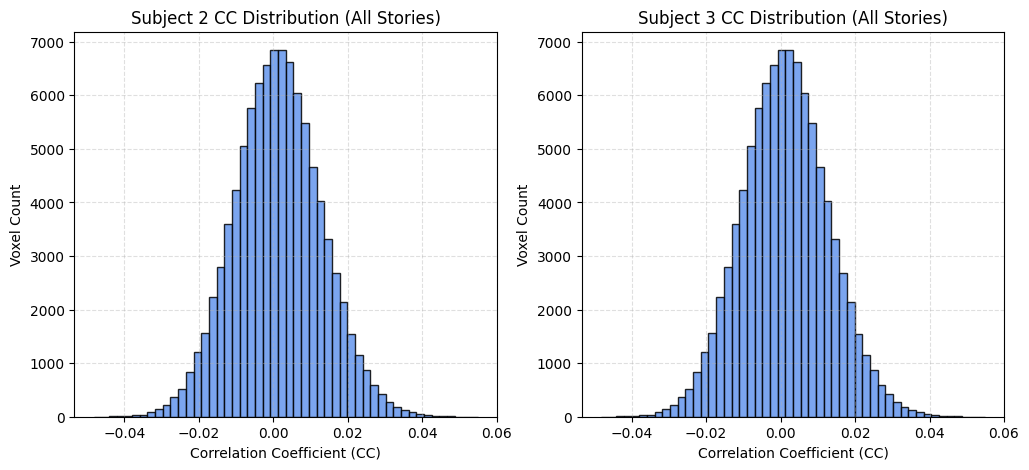
\includegraphics{cc_bow.png}
\caption{BoW CC Distribution for Subject 2 and 3}
\end{figure}

Although overall CCs are relatively low due to the sparsity and high
dimensionality of BoW, we observe a few voxels with moderate predictive
performance.

\hypertarget{glove-model-results}{%
\subsubsection{4.3 GloVe Model Results}\label{glove-model-results}}

We next evaluated the \textbf{GloVe embeddings}, using a 100-dimensional
pretrained vector for each word, followed by downsampling, trimming, and
delaying. We trained models using \textbf{voxel-specific alpha values}
estimated from bootstrap ridge regression.

\textbf{Subject 2 (GloVe + bootstrap\_ridge + valphas):}

\begin{itemize}
\item
  \textbf{Mean CC}: 0.0129
\item
  \textbf{Median CC}: 0.0104
\item
  \textbf{Top 1\% CC}: 0.0702
\item
  \textbf{Top 5\% CC}: 0.0462
\end{itemize}

\textbf{Subject 3 (GloVe + bootstrap\_ridge + valphas):}

\begin{itemize}
\item
  \textbf{Mean CC}: 0.0181
\item
  \textbf{Median CC}: 0.0151
\item
  \textbf{Top 1\% CC}: 0.0787
\item
  \textbf{Top 5\% CC}: 0.0550
\end{itemize}

\begin{figure}
\centering
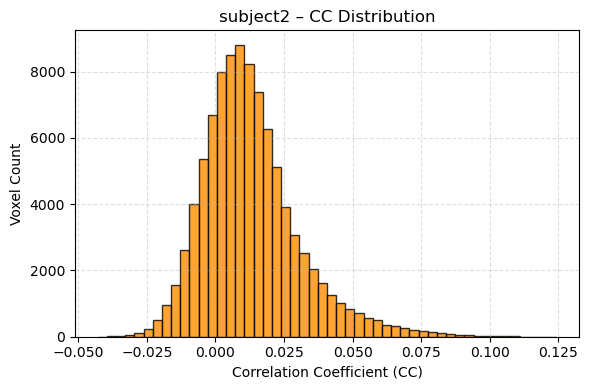
\includegraphics{cc_glove1.png}
\caption{Glove CC Distribution for Subject 2}
\end{figure}

\begin{figure}
\centering
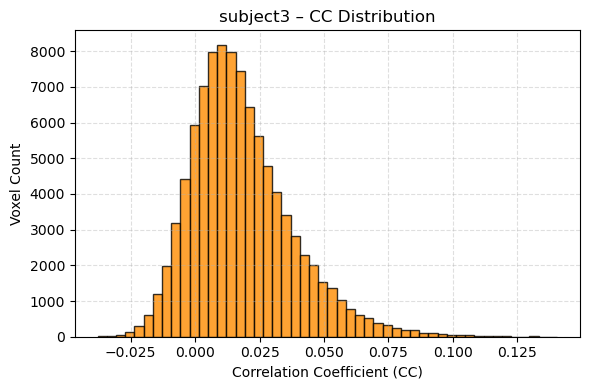
\includegraphics{cc_glove2.png}
\caption{Glove CC Distribution for Subject 3}
\end{figure}

These results show a clear improvement over BoW, reflecting GloVe's
semantic compactness and reduced dimensionality.

\hypertarget{word2vec-model-results}{%
\subsubsection{4.4 Word2Vec Model
Results}\label{word2vec-model-results}}

\hypertarget{detailed-cc-distribution-analysis}{%
\subsubsection{4.5 Detailed CC Distribution
Analysis}\label{detailed-cc-distribution-analysis}}

To better understand model behavior across voxels, we examined the full
distribution of CCs. We found that:

\begin{itemize}
\item
  The distribution is unimodal and slightly right-skewed, with most
  voxels near zero.
\item
  A small subset of voxels show moderate CCs, suggesting localized
  regions that respond reliably to semantic features.
\item
  \textbf{Subject 3 consistently shows better model fit across all
  voxels} compared to Subject 2.
\end{itemize}

These patterns suggest that GloVe features generalize well and may
better reflect the semantic structure encoded in cortical regions.

\hypertarget{stability-analysis}{%
\subsubsection{4.6 Stability Analysis}\label{stability-analysis}}

We conducted a \textbf{stability analysis} by re-evaluating performance
on random subsets of voxels using the pretrained valphas.

\textbf{Subject 2 Stability (GloVe):}

\begin{longtable}[]{@{}lllll@{}}
\toprule
Subset Size & Mean CC & Median CC & Top 1\% CC & Top 5\% CC \\
\midrule
\endhead
1,000 & 0.0137 & 0.0101 & 0.0819 & 0.0485 \\
10,000 & 0.0129 & 0.0104 & 0.0688 & 0.0458 \\
20,000 & 0.0130 & 0.0105 & 0.0693 & 0.0463 \\
\bottomrule
\end{longtable}

\textbf{Subject 3 Stability (GloVe):}

\begin{longtable}[]{@{}lllll@{}}
\toprule
Subset Size & Mean CC & Median CC & Top 1\% CC & Top 5\% CC \\
\midrule
\endhead
1,000 & 0.0179 & 0.0153 & 0.0774 & 0.0546 \\
10,000 & 0.0182 & 0.0153 & 0.0794 & 0.0545 \\
20,000 & 0.0181 & 0.0152 & 0.0784 & 0.0546 \\
\bottomrule
\end{longtable}

\begin{figure}
\centering
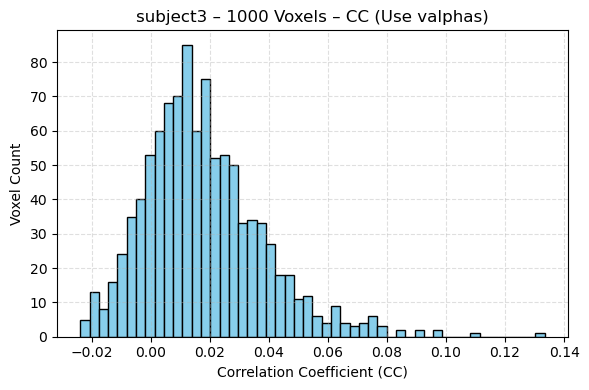
\includegraphics{vox_glove4.png}
\caption{1K Voxel Stability for Subject 3}
\end{figure}

\begin{figure}
\centering
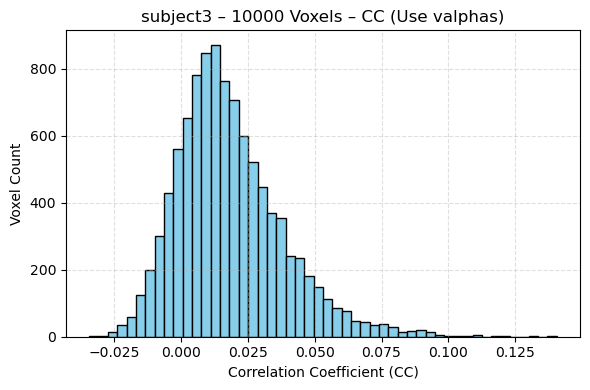
\includegraphics{vox_glove5.png}
\caption{10K Voxel Stability for Subject 3}
\end{figure}

\begin{figure}
\centering
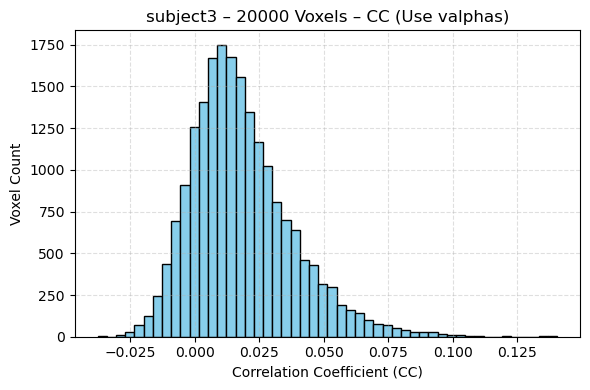
\includegraphics{vox_glove6.png}
\caption{20K Voxel Stability for Subject 3}
\end{figure}

These results confirm the robustness of the model's predictive ability,
particularly for Subject 3. Even when reducing the number of voxels by
90\%, the overall distribution and top percentile performance remain
stable.

\hypertarget{interpretation-and-scientific-implications}{%
\subsubsection{4.7 Interpretation and Scientific
Implications}\label{interpretation-and-scientific-implications}}

Our results show that GloVe embeddings outperform Bag-of-Words in
predicting brain activity, consistent with the notion that semantic
representations are more informative than word counts. Subject 3
consistently achieved higher CCs, suggesting either a better
signal-to-noise ratio in the data or greater alignment with the semantic
features.

The detailed voxel-wise distribution also implies that language-related
processing is spatially localized: only a subset of voxels reliably
encode linguistic information. By identifying these voxels, we can begin
mapping the cortical regions most involved in semantic comprehension.

A reasonable PCS-aligned interpretation criterion might be to define
``active'' voxels as those within the top 1\% of CCs (i.e., CC
\textgreater{} \textasciitilde0.07), which balances statistical
reliability with biological plausibility.

\hypertarget{summary}{%
\subsubsection{4.8 Summary}\label{summary}}

\begin{itemize}
\tightlist
\item
  Ridge regression with GloVe embeddings yields substantially higher
  prediction accuracy than Bag-of-Words.
\item
  Subject 3 shows consistently better model performance than Subject 2.
\item
  The model is stable across varying voxel subsets, especially in
  GloVe-based analyses.
\item
  Top-performing voxels exhibit strong semantic sensitivity, supporting
  the use of encoding models to probe language representation in the
  brain.
\end{itemize}

    \hypertarget{bibliography}{%
\section{5. Bibliography}\label{bibliography}}

Shailee Jain and Alexander Huth. ``Incorporating Context into Language
Encoding Models for fMRI''. In: Advances in Neural Information
Processing Systems. Ed. by S. Bengio et al.~Vol. 31. Curran Associates,
Inc., 2018. url:
https://proceedings.neurips.cc/paper\_files/paper/2018/file/
f471223d1a1614b58a7dc45c9d01df19-Paper.pdf.

    \hypertarget{a.-academic-honesty}{%
\section{A. Academic Honesty}\label{a.-academic-honesty}}

\hypertarget{a.1-statement}{%
\subsubsection{A.1 Statement}\label{a.1-statement}}

We confirm that this report represents the collaborative work of our
entire group. All analysis methods and procedures were jointly designed
and executed. The text, figures, and research process have been
documented transparently to ensure reproducibility. Any references to
others' work have been properly cited. Research integrity is fundamental
to academic progress. While scholarship builds on prior knowl- edge,
every study must uphold truthfulness, reliability, and originality.
Irreproducible methods or unattributed work undermine trust and devalue
collective scholarly efforts. As a team, we affirm our commitment to
transparency, respect for intellectual contributions, and accountability
for main- taining ethical standards. Each member has ensured that our
work is original, properly cited, and advances understanding of Arctic
cloud detection through honest collaboration.

\hypertarget{a.2-llm-usage}{%
\subsubsection{A.2 LLM Usage}\label{a.2-llm-usage}}

ChatGPT was used as a coding assistant for syntax validation and
visualization enhancements, specifically for refining graph color
schemes. All analytical decisions, model implementations, and
evaluations were performed independently by the authors.


    % Add a bibliography block to the postdoc
    
    
    
\end{document}
